\chapter{The \Hgg event categorisation}\label{app:event_categorisation}

% \vspace{-.5cm}
\section{ML classifier input features}
Table~\ref{tab:categorisation_input_features} provides a full list of the input features, $\vec{x}$, used for the ML classifiers in the \Hgg analysis. The definitions of the less obvious features are provided below:

\begin{itemize}
    \item $\Delta$: refers to the difference between two quantities. For example, $\Delta\eta_{jj}$, is the difference in pseudorapidity between the two jets in the dijet system.
    \item $\sigma_{RV}$: per-event relative diphoton mass resolution estimate, under the hypothesis that the mass is reconstructed with the correct primary vertex. 
    \item $\sigma_{WV}$: per-event relative diphoton mass resolution estimate, under the hypothesis that the mass is reconstructed with the incorrect primary vertex.
    \item $C_{\gamma\gamma}$: dijet centrality defined as,
    \begin{equation}
        C_{\gamma\gamma} = {\rm{exp}} \Bigg( - \frac{4}{(\eta_1-\eta_2)^2} \Big( \eta_{\gamma\gamma} - \frac{\eta_1+\eta_2}{2} \Big)^2 \Bigg),
    \end{equation}
    \noindent
    where $\eta_1$, $\eta_2$, and $\eta_{\gamma\gamma}$, are the lead jet, sublead jet and diphoton $\eta$, respectively. This quantity is extremely useful for identifying the VBF-like topology with two forward jets.
    \item $\cos{\theta^*}$: cosine of the difference of two angles, namely the diphoton system in the diphoton-dijet centre-of-mass frame, and the diphoton-dijet system in the lab frame.
    \item $H_T$: scalar sum of the transverse energy of all reconstructed particles in the event.
    \item $m_T$: transverse mass, defined as,
    \begin{equation}
        m_T = \sqrt{2p_T^\ell\met(1-\cos{\Delta\phi_{\ell,\met}})},
    \end{equation}
    \noindent
    where $\Delta\phi_{\ell,\met}$ is the azimuthal separation between the lepton and \met.
    \item $\theta_H$: angle between the two photons in the diphoton rest frame.
    \item DeepJet and DeepCSV: refer to the algorithm used for the CMS b tagging.
    \item Pixel seed veto: flag to veto photon objects with corresponding hits in the innermost tracker layers. Useful for rejecting electrons which can mimic the photon signal.
    \item $Y_{\gamma\gamma}$: rapidity of the diphoton.
    \item $N_{X}$: the multiplicity of object, $X$. For example, $N_{\rm{jets}}$, is the number of reconstructed jets in the event.
    \item DNN scores in the ttH background rejection BDTs: additional DNNs are trained with ttH signal events against one source of background only. These discriminants first entered in the \Hgg analysis of Ref.~\cite{Sirunyan:2020sum}, which specifically targets the ttH production mode. Three DNNs are trained in total: one for each of the $\gamma\gamma$+jets and $tt+\gamma\gamma$ backgrounds in the hadronic channel, and one for the $tt+\gamma\gamma$ background in the leptonic channel. The performance of these DNNs benefits from the high number of simulated events on which to train, as well as the fact that both of the considered backgrounds are well modelled in simulation. Importantly, the DNNs use a combination of high-level and lower-level input features, where the latter includes the full four-momentum vectors of the reconstructed objects in the event. Adding this low-level information directly into the background rejection BDTs does not improve their performance. However, using a DNN as an intermediate step and feeding the output score of the DNN into the BDT, allows the low-level information to be utilised effectively.
    \item Top tagger BDT score: a ML algorithm developed for the analysis in Ref.~\cite{Sirunyan:2017wif}, is used to distinguish events with top quarks decaying to three jets, from events that do not contain top quarks. The algorithm is trained on jet triplets from the simulation of tt production events, with input features related to the event kinematics, b tag scores, and the jet shape. The signal is defined as a jet triplet which is matched at truth-level to a top quark, and the background is taken as random jet triplets.
\end{itemize}

\begin{table}[htb]
    \caption[Input features to the \Hgg event classifiers]{Input features to the ML event classifiers used in the \Hgg analysis. Photons, jets, b-tagged jets and leptons are labelled as $\gamma$, $j$, $bj$, and $\ell$, respectively,  and the numbers represent the $p_T$-ordered list of the respective objects e.g. $\gamma 1$ corresponds to the leading photon. The diphoton (dijet) variables are labelled by $\gamma\gamma$ ($jj$). In the final two classifiers, $\rm{fwd}$ corresponds to the jet with the highest $|\eta|$ value, which provides a useful handle on identifying events originating from tHq production. Definitions of the less obvious input features are provided in the main text of this Appendix.}
    \label{tab:categorisation_input_features}
    % \vspace{.5cm}
    \centering
    \scriptsize
    \renewcommand{\arraystretch}{3}
    \setlength{\tabcolsep}{6pt}
    % \hspace*{-0.5cm}
    \begin{tabular}{l|m{11cm}<{\centering}}
    \hline
    Discriminant/Classifier & Input features, $\vec{x}$ \\ \hline
    ggH BDT & $p_T^{\gamma 1/\gamma 2}/m_{\gamma\gamma}$, $\eta^{\gamma 1/\gamma 2}$, $\cos{\Delta\phi_{\gamma\gamma}}$, $\gamma 1/\gamma 2$ ID BDT scores, $\sigma_{RV}$, $\sigma_{WV}$, vertex probability BDT score, $p_T^{\gamma\gamma}$, $N_{\rm{jets}}$, $m_{jj}$, $\eta^{j1/j2/j3}$, $j1/j2/j3$ pile-up identification BDT scores, $\Delta\phi_{\gamma\gamma,j1/j2/j3}$, $\Delta\eta_{\gamma\gamma,j1/j2/j3}$ \\ \hline
    
    Diphoton BDT & $p_T^{\gamma 1/\gamma 2}/m_{\gamma\gamma}$, $\eta^{\gamma 1/\gamma 2}$, $\cos{\Delta\phi_{\gamma\gamma}}$, $\gamma 1/\gamma 2$ ID BDT scores, $\sigma_{RV}$, $\sigma_{WV}$, vertex probability BDT score \\ \hline
    
    Dijet BDT & $p_T^{\gamma 1/\gamma 2}/m_{\gamma\gamma}$, $p_T^{\gamma\gamma}/m_{\gamma\gamma}$, $\cos{\Delta\phi_{\gamma\gamma}}$, $p_T^{j1/j2}$, $m_{jj}$, $\Delta\phi_{\gamma\gamma,jj}$, min($\Delta R_{\gamma,j}$), $C_{\gamma\gamma}$, $|\Delta\eta_{jj}|$, $\Delta\phi_{jj}$ \\ \hline
    
    VH hadronic BDT & $p_T^{\gamma 1/\gamma 2}/m_{\gamma\gamma}$, $p_T^{j1/j2}$, $\eta^{j1/j2}$, $m_{jj}$, $|\Delta\eta_{jj}|$, $\cos{\theta^*}$ \\ \hline    
    
    VH MET BDT & $p_T^{\gamma 1/\gamma 2}/m_{\gamma\gamma}$, $\eta^{\gamma 1/\gamma 2}$, $\cos{\Delta\phi_{\gamma\gamma}}$, max/min $\gamma$ ID BDT scores, \met, $H_T$, $N_{\rm{jets}}$, $p_T^{j1}$, max jet b-tag score (deepCSV), $\Delta\phi_{\gamma\gamma,\met}$, min($\Delta\phi_{\met,j})$, $(p_T^{\gamma\gamma}-\met)/p_T^{\gamma\gamma}$ \\ \hline
    
    WH leptonic BDT & $p_T^{\gamma 1/\gamma 2}/m_{\gamma\gamma}$, $\eta^{\gamma 1/\gamma 2}$, $\cos{\Delta\phi_{\gamma\gamma}}$, max/min $\gamma$ ID BDT scores, $\gamma 1/\gamma 2$ pixel seed veto, $p_T^\ell$, $\eta^\ell$, $\Delta R_{\gamma 1/\gamma 2,\ell}$, $\Delta\theta_{\gamma\gamma,\ell}$, \met, $m_T$, $N_{\rm{jets}}$, $p_T^{j1}$, $j1/j2$ b-tag score (deepCSV) \\ \hline
    
    ZH leptonic BDT & $p_T^{\gamma 1/\gamma 2}/m_{\gamma\gamma}$, $\eta^{\gamma 1/\gamma 2}$, $\cos{\Delta\phi_{\gamma\gamma}}$, max/min $\gamma$ ID BDT scores, $\gamma 1/\gamma 2$ pixel seed veto, $p_T^{\ell 1/\ell 2}$, $\eta^{\ell 1/\ell 2}$, $\Delta R_{\gamma 1/\gamma 2,\ell 1/\ell 2}$, $\Delta\theta_{\gamma\gamma,\ell\ell}$, $m_{\ell\ell}$, $N_{\rm{jets}}$, $p_T^{j1}$, $j1$ b-tag score (deepCSV) \\ \hline

    ttH hadronic BDT & $p_T^{\gamma 1/\gamma 2}/m_{\gamma\gamma}$, $\eta^{\gamma 1/\gamma 2}$, max/min $\gamma$ ID BDT scores, $\gamma 1/\gamma 2$ pixel seed veto, $p_T^{\gamma\gamma}/{m_{\gamma\gamma}}$, $Y_{\gamma\gamma}$, $|\cos{\Delta\phi_{\gamma\gamma}}|$, $\Delta R_{\gamma\gamma}$, $\cos{\theta_H}$, $p_T^{j1/j2/j3/j4}$, $\eta^{j1/j2/j3/j4}$, $j1/j2/j3/j4$ b-tag score (DeepJet), max/min b-tag score, $N_{\rm{jets}}$, $H_T$, \met, DNN scores: ttH vs tt$\gamma\gamma$ (had) and ttH vs $\gamma\gamma$+jets (had), Top tagger BDT score \\ \hline
    
    ttH leptonic BDT & $p_T^{\gamma 1/\gamma 2}/m_{\gamma\gamma}$, $\eta^{\gamma 1/\gamma 2}$, max/min $\gamma$ ID BDT scores, $\gamma 1/\gamma 2$ pixel seed veto, $p_T^{\gamma\gamma}/{m_{\gamma\gamma}}$, $Y_{\gamma\gamma}$, $|\cos{\Delta\phi_{\gamma\gamma}}|$, $\Delta R_{\gamma\gamma}$, $\cos{\theta_H}$, $p_T^{j1/j2/j3}$, $\eta^{j1/j2/j3}$, $j1/j2/j3$ b-tag score (DeepJet), max/min b-tag score, $N_{\rm{jets}}$, $H_T$, \met, $p_T^\ell$, $\eta^\ell$, $N_{\rm{leptons}}$ (tight ID), DNN scores: ttH vs tt$\gamma\gamma$ (lep) \\ \hline
    
    tHq leptonic BDT & $p_T^{\gamma 1/\gamma 2}/m_{\gamma\gamma}$, $\eta^{\gamma 1/\gamma 2}$, max/min $\gamma$ ID BDT scores, $\gamma 1/\gamma 2$ pixel seed veto, $N_{\rm{jets}}$, $N_{\rm{bjets}}$, $N_{\rm{jets}}$ with $|\eta|<1$, $p_T^{j1/j2/j3}$, $\eta^{j1/j2/j3}$, $p_T^{bj1/bj2/bj3}$, $\eta^{bj1/bj2/bj3}$, $p_T^{\rm{fwd}}$, $\eta^{\rm{fwd}}$, $\Delta\phi_{\gamma 1/\gamma 2,j1}$, $\Delta\phi_{\gamma 1/\gamma 2,\ell}$, $\Delta\phi_{\gamma 1/\gamma 2,bj1}$, $\Delta\phi_{\gamma 1/\gamma 2,{\rm{fwd}}}$, $p_T^\ell$, $\eta^\ell$ \\ \hline
    
    Top DNN & $p_T^{\gamma 1/\gamma 2}/m_{\gamma\gamma}$, $\eta^{\gamma 1/\gamma 2}$, max/min $\gamma$ ID BDT scores, $\gamma 1/\gamma 2$ pixel seed veto, $p_T^{\gamma\gamma}/{m_{\gamma\gamma}}$, $Y_{\gamma\gamma}$, $|\cos{\Delta\phi_{\gamma\gamma}}|$, $\Delta R_{\gamma\gamma}$, $\cos{\theta_H}$, $p_T^{j1/j2/j3}$, $\eta^{j1/j2/j3}$, $j1/j2/j3$ b-tag score (DeepJet), max/min b-tag score, $N_{\rm{jets}}$, $H_T$, \met, $p_T^\ell$, $\eta^\ell$, $N_{\rm{leptons}}$ (tight ID), $p_T^{\rm{fwd}}$, $\eta^{\rm{fwd}}$, $\ell 1/\ell 2$ charge \\
    \hline
\end{tabular}
    % \hspace*{-0.5cm}
\end{table}

\begin{figure}[htb!]
  \centering
  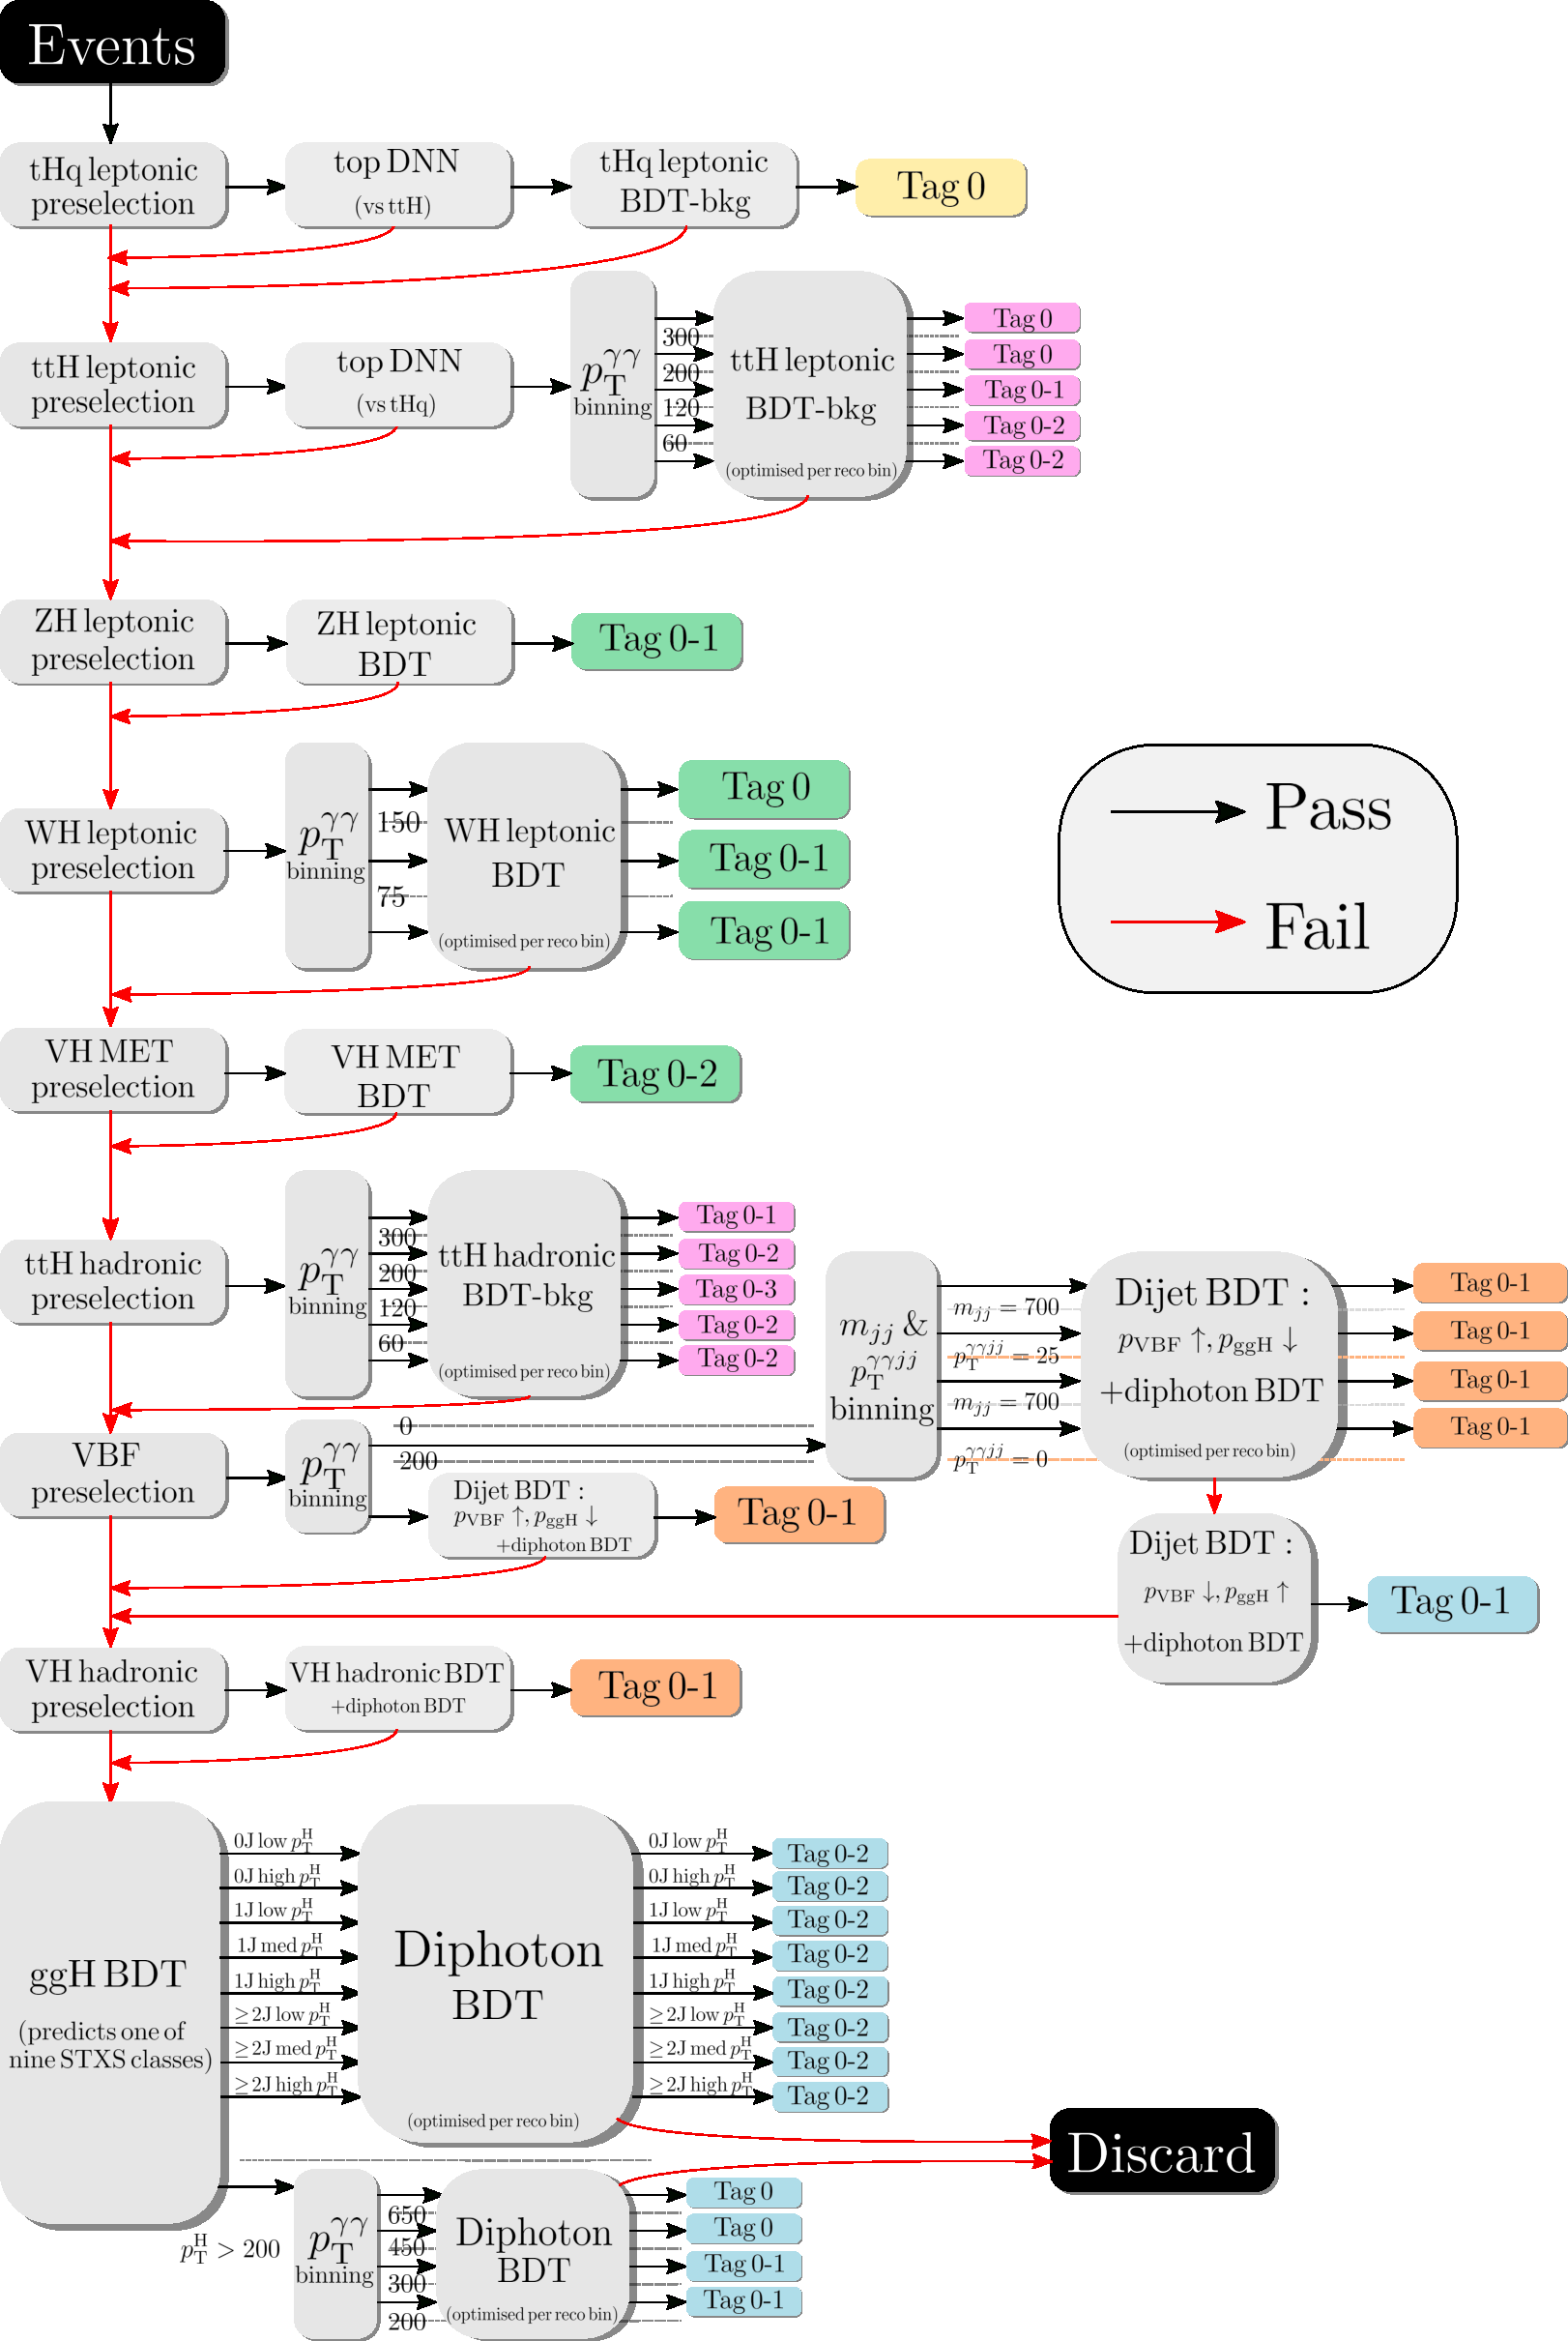
\includegraphics[width=.9\textwidth]{Figures/app_categorisation/categorisation_schematic.pdf}
  \caption[Schematic of the \Hgg event categorisation]
  {
    A schematic of the event categorisation in the \Hgg analysis. Reconstructed events passing the trigger selection are required to pass the photon pre-selection criteria. Those that do, enter the top left of the diagram. In the schematic, black and red lines signify events passing and failing the relevant criteria, respectively. Events that do not end up in any analysis category (coloured boxes) are discarded from the analysis.
  }
  \label{fig:categorisation_schematic}
\end{figure}